\begin{frame}{Theory: Topological insulator}
	2005 Kane and Mele found another class of material: \\the topological insulator (TI).
	\\
	\begin{columns}
		\begin{column}<2->{0.33\linewidth}
			spin-orbit coupling
		\end{column}
		\hspace{-1cm}
		\begin{column}<3->{0.33\linewidth}
			$\rightarrow$ band inversion
		\end{column}
		\hspace{-1.2cm}
		\begin{column}<4->{0.33\linewidth}
			$\rightarrow$ Dirac cone
		\end{column}
	\end{columns}
	\begin{columns}
		\begin{column}<4->{.5\linewidth}
			\begin{figure}
				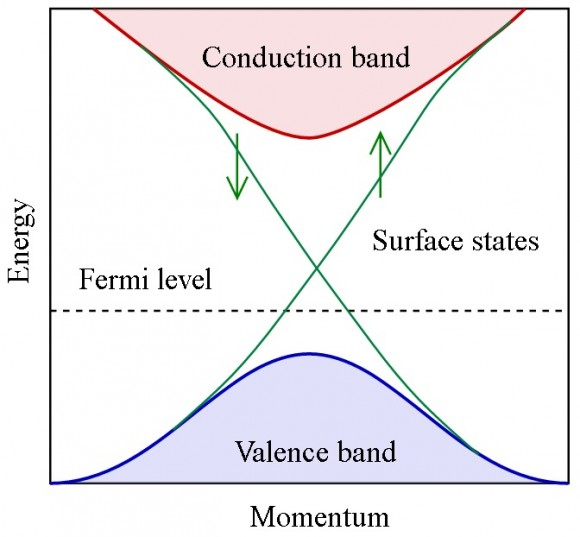
\includegraphics[width=\textwidth]{andere_bilder/band_structure_top_insulator}
			\end{figure}
		\end{column}
		\begin{column}{.5\linewidth}
			\begin{block}<5->{2D TI: }
			have quantum spin edge states found in graphene and HgTe quantum wells.
			\end{block}
			\begin{block}<6->{3D TI: }
			strong and weak ones \\
			HgTe is semi metal but under strain $\Gamma_6$ and $\Gamma_8$ bands can close up at Fermi level. 
			\end{block}
		\end{column}
	\end{columns}
	
\end{frame}

\begin{frame}{Theory: Crystal and surface description part 1}

	\begin{block}{Translation Vector: $\boldsymbol{R}_i = x_i \boldsymbol{a}_1 + y_i \boldsymbol{a}_2 + z_i \boldsymbol{a}_3$}
		contains basis for lattice forming a unit cell. \\
		Smallest primitive unit cell is the Wigner Seitz cell.
	\end{block}
	\begin{columns}
		\begin{column}<2->{0.3\linewidth}
			Bravais lattice  
		\end{column}
	\end{columns}
	\begin{columns}
		\begin{column}<3->{0.5\linewidth}
			fcc lattice with two atomic basis 
		\end{column}
		\hspace{-1cm}
		\begin{column}<4->{0.55\linewidth}
			$\rightarrow$ diamond or zinc-blende structure 
		\end{column}
	\end{columns}
	\hfill
	\begin{columns}<5->
		\begin{column}{.25\linewidth}
			\centering
			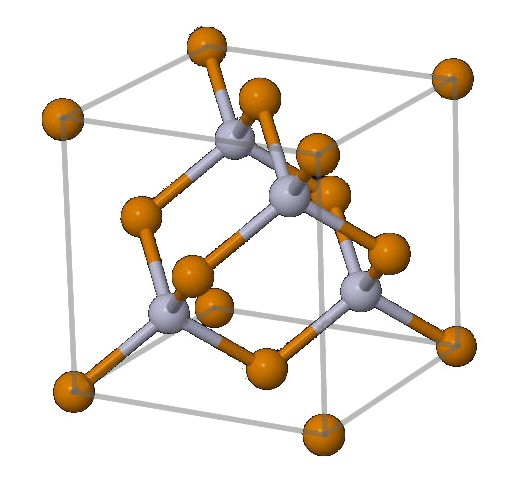
\includegraphics[width=\linewidth]{andere_bilder/zinc_blende}
		\end{column}
%		\hspace{-.7cm}
		\begin{column}{.25\linewidth} 
		\scriptsize{
			\centering
			\begin{tabular}{c c c c} 
				\hline
				& \textbf{x} & \textbf{y} & \textbf{z}\\ 
				\hline 
				\vspace{0.2cm} 
				$\boldsymbol{a}_1$ & 0 & $\frac{a}{2}$ & $\frac{a}{2}$ \\
				\vspace{0.2cm}
				$\boldsymbol{a}_2$ & $\frac{a}{2}$ & 0 & $\frac{a}{2}$ \\
				\vspace{0.2cm}
				$\boldsymbol{a}_3$ & $\frac{a}{2}$ & $\frac{a}{2}$ & 0 \\
%			\end{tabular}	
%		\end{minipage}
%		\\
%		\begin{column}[c]{.33\linewidth}
%			\begin{tabular}{c c c c} 
%				\hline
%				& \textbf{x} & \textbf{y} & \textbf{z}\\ 
				\hline 
				\vspace{0.2cm}
				Te & 0 & 0 & 0 \\
				\vspace{0.2cm}
				Hg & $\frac{a}{4}$ & $\frac{a}{4}$ & $\frac{a}{4}$
			\end{tabular}
		}
		\end{column}
		\begin{column}<6->{.5\linewidth}
			\begin{minipage}{\linewidth}
			Miller indices: $(hkl)$
			\begin{equation*}
			h : k : l = \frac{1}{x} : \frac{1}{y} : \frac{1}{z}
			\end{equation*}
			\end{minipage}
			\\
			\begin{minipage}{\linewidth}
			\centering
			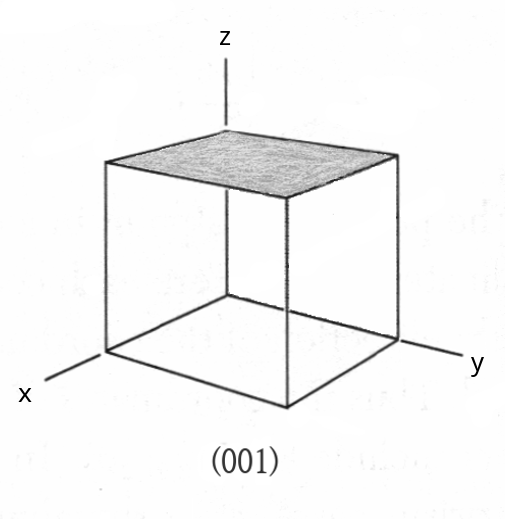
\includegraphics[width=.5\linewidth]{extrabilder_fuer_vortrag/millersche_indizes_001}
			\end{minipage}
		\end{column}
	\end{columns}
\end{frame}

\begin{frame}{Theory: Crystal and surface description part 2}
	Basis for (001) direction of zinc-blende structure: 
	\begin{columns}
		\hspace{-1cm}
		\begin{column}<2->{.25\linewidth}
			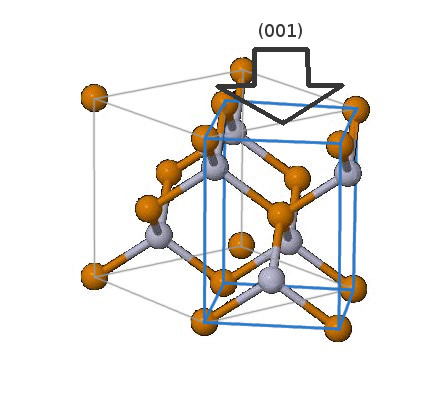
\includegraphics[width=1.2\linewidth]{andere_bilder/zinc_blende_45degree.jpg}
		\end{column}
		\hspace{-1cm}
		\begin{column}<2->{.2\linewidth}\scriptsize{
			\begin{tabular}{c c c c} 
				\hline
				& \textbf{x} & \textbf{y} & \textbf{z}\\ 
				\hline 
				\vspace{0.2cm} 
				$\boldsymbol{a}_1$ & $\frac{a}{\sqrt{2}}$  & 0 & 0 \\
				\vspace{0.2cm}
				$\boldsymbol{a}_2$ & 0 & $\frac{a}{\sqrt{2}}$ & 0 \\
				\vspace{0.2cm}
				$\boldsymbol{a}_3$ & 0 & 0 & $a$ 
			\end{tabular}
		}	
		\end{column}
		\begin{column}<2->{.3\linewidth}\scriptsize{
			\begin{tabular}{c c c c} 
				\hline
				& \textbf{x} & \textbf{y} & \textbf{z}\\ 
				\hline
				\vspace{0.2cm} 
				Te & 0 & 0 & 0 \\
				\vspace{0.2cm}
				Hg & $\frac{a}{2\sqrt{2}}$ & 0 & $\frac{a}{4}$ \\
				\vspace{0.2cm}
				Te & $\frac{a}{2\sqrt{2}}$ & $\frac{a}{2\sqrt{2}}$ & $\frac{a}{2}$ \\
				\vspace{0.2cm}
				Hg & 0 & $\frac{a}{2\sqrt{2}}$ & $\frac{3a}{4}$
			\end{tabular}
		}
		\end{column}
	\end{columns}
	\begin{columns}
		\begin{column}<3->{.6\linewidth}
			Reciprocal lattice: $e^{i\boldsymbol{K}\boldsymbol{R}} = 1$\\
			$\boldsymbol{K}$ is reciprocal translation vector.\\
			First Brillouin zone (BZ) is Wigner Seitz cell for reciprocal space.\\
			Super symmetrical points:\vspace{-.3cm}
			\begin{align*}
			\overline{\Gamma}&= 0;&
			\overline{\text{J}} &= \frac{1}{2} \boldsymbol{b}_1 ;&
			\overline{\text{K}}&= \frac{1}{2} \boldsymbol{b}_1 + \frac{1}{2} \boldsymbol{b}_2 
			\end{align*}
		\end{column}
		\begin{column}<3->{.4\linewidth}
			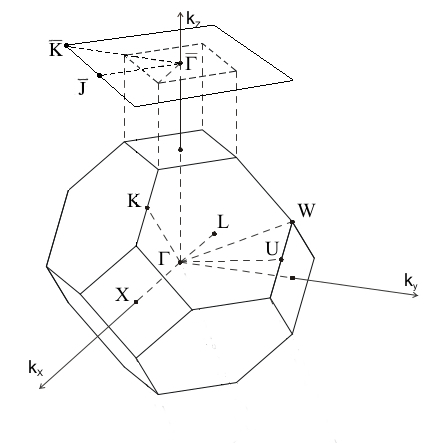
\includegraphics[width=\linewidth]{andere_bilder/brillouin_zone_001_2}
		\end{column}
	\end{columns}
\end{frame}

\begin{frame}{Theory: Surface modeling}
	\begin{columns}
		\begin{column}{.86\linewidth}
			\begin{block}{Termination}
				Two surfaces with symmetric Hg-Hg, Te-Te terminations or antisymmetric Te-Hg terminations.\\
				Add hydrogen atoms in order to saturate dangling bonds. 
			\end{block}
			\begin{block}<2->{Number of layers}
				Atoms with same z component are in the same layer. \\
				Odd for symmetric, even for antisymmetric termination.\\
				I studied 3 different thicknesses for each termination.
			\end{block}
			\begin{block}<3->{Supercell approach}
				Infinite repetition only possible in all directions.\\
				In order to avoid interactions between slabs in $k_z$ direction: add vacuum space. 
			\end{block}
		\end{column}
		\begin{column}<3->{0.14\linewidth} 
			\centering
			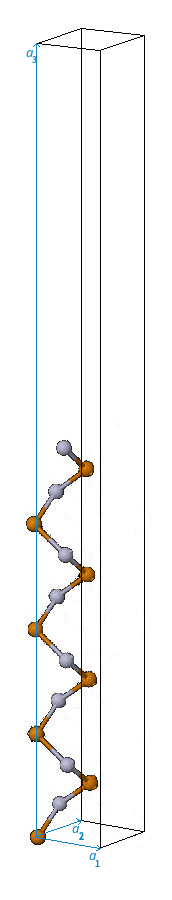
\includegraphics[width=\linewidth]{andere_bilder/hgte_16layer_supercell_2.jpg} 
		\end{column} 
	\end{columns}
\end{frame}

\begin{frame}{Theory: DFT and SOC}
	blub
\end{frame}

%%% Local Variables:
%%% mode: latex
%%% TeX-master: "main_BA2_Vortrag.tex"
%%% End: